This section treats each ecosystem in turn with one subsection per
ecosystem. Within each ecosystem, we present per-server
measurements, the source-code location of the chunked-decoder
dispatch, the dominant profile hot path under attack, and a brief
discussion of why the server is in the verdict class it occupies.
Numerical results are auto-extracted from \texttt{data/wave*.json};
the full reproducer is at \texttt{wave\{1,2\}/<ecosystem>/repro/}.

A 17-dimension per-framework deep dive (versions, parser
provenance, source map, profile, mitigations, regression, etc.)
is in progress and will appear in the extended version of this
paper.

\subsection{Python (Wave 1 + extended Wave 2)}
\label{sec:pf-python}

\paragraph{ASGI servers.}
The Python ASGI ecosystem has five widely-deployed servers.
\fwid{uvicorn} 0.32.1 with the \fwid{httptools} backend is the
fastest in our sample (\SI{2.1}{\micro\second}/chunk); the
\fwid{h11} backend on the same uvicorn is \SI{5}{\micro\second}.
\fwid{daphne} (Twisted-based, used by Django Channels) sits at
\SI{2.5}{\micro\second}. \fwid{hypercorn} h11 backend is
\SI{7.5}{\micro\second}. \fwid{granian} (Rust core via PyO3) is
the slowest at \SI{14.4}{\micro\second}/chunk; the Rust-to-Python
bridge cost per chunk dominates its measurement.

All five emit one ASGI \fname{\{type: "http.request"\}} receive
event per h11 / httptools data event. The relevant code paths are
\fname{uvicorn/protocols/http/h11\_impl.py:257-261} (uvicorn h11
backend) and \fname{uvicorn/protocols/http/httptools\_impl.py:301}
(uvicorn httptools backend). None aggregate.

\paragraph{WSGI / hand-rolled servers (Wave 2).}
\fwid{gunicorn} sync workers (Django/Flask production default)
register \SI{2.7}{\micro\second}/chunk on the fast Mode A but
super-linear scaling under heavier loads; the hot path is
\fname{gunicorn/http/body.py:77 parse\_chunk\_size}. \fwid{waitress}
3.0.2 reaches \SI{18.4}{\micro\second}/chunk under Mode A with
similar super-linear behavior. \fwid{tornado} 6.4.2 is comparable.
None of the three exhibit a clean BATCHES-CORRECTLY pattern: while
gunicorn's `wsgi.input.read()` does fully buffer at the handler
boundary, the chunked decoder underneath still loops one Python
function call per chunk before the buffered IO returns.

\subsection{Go}
\label{sec:pf-go}

The Go standard library's \fname{net/http} chunked decoder lives
at \fname{net/http/internal/chunked.go}; its
\fname{chunkedReader.beginChunk} runs one
\fname{bufio.Reader.fill} call per chunk header. The hot path
shows 73\% of cumulative time in
\fname{syscall.Read} + \fname{bufio.fill}: one syscall per chunk.
\fwid{gin} is indistinguishable because it uses the stdlib decoder
unchanged. Both servers measure
\SI{13.4}{\micro\second}/chunk under Mode B.

Go has shipped one adjacent CVE in this family
(CVE-2023-39326~\cite{cve_2023_39326_go}: a chunk-extension cost
cap), but the raw-chunk-count amplification we measure is
explicitly not covered by the existing cap.

\subsection{Rust}
\label{sec:pf-rust}

\fwid{hyper}'s internal chunked decoder
(\fname{ChunkedState::Body}) yields one \fname{Frame::data(Bytes)}
per parsed chunk. \fwid{axum} (built on \fname{hyper}) sits at
\SI{4.3}{\micro\second}/chunk. \fwid{actix-web} (different
concurrency model: Actix actor system on top of Tokio) uses its
own \fname{actix-http PayloadDecoder} but the same one-frame-per-
chunk pattern; it measures \SI{2.3}{\micro\second}/chunk.

The Rust ecosystem also provides the closest thing to public
prior art on this class: hyper issue \#4008~\cite{hyper_4008}
was opened as an RFC for built-in chunked request limits and
closed \fname{not\_planned} on 2026-01-12 with the labelled state
\fwid{S-waiting-on-author}. The maintainer's closing comment, in
substance, was that the maintainer was personally skeptical of
the described problem ("if as a developer my server does heavy
work, I need to design it properly") and encouraged the reporter
to maintain a limit-helpers crate as a separate library.
The proposed \fname{BodyExt::limit\_chunks(N)} helper was not
shipped in \fname{http\_body\_util}. We characterize this as a
feature-scope decision by a maintainer skeptical of the threat
framing; we do not characterize it as a deliberate security
position.

\subsection{Node.js (the four QUADRATIC servers)}
\label{sec:pf-node}

Node's built-in \fname{http.Server} measures
\SI{1128}{\micro\second}/chunk at $N{=}\num{250000}$ (Mode A,
measured), with a measured scaling exponent of $\sim 1.7$--$2.0$
in the $N \in \{\num{50000}, \num{100000}, \num{250000}\}$ range.
\fwid{express} 5.x and \fwid{fastify} 5.x extrapolate from
smaller cells (measured $N{=}\num{50000}$ and $N{=}\num{100000}$)
to $\sim 324$ s and $\sim 339$ s at $N{=}\num{250000}$
respectively\footnote{We mark extrapolated cells with an asterisk
in Table~\ref{tab:matrix}; the underlying $N{=}\num{50000}$ and
$N{=}\num{100000}$ data points were measured directly.}. The
framework layer adds essentially nothing because all three use
the same underlying \fname{http.Server} + \fname{llhttp}
substrate.

The profile hot path is:
\fname{llhttp on\_body} (C) -> \fname{parserOnBody}
(\fname{node:\_http\_common:128}) ->
\fname{readableAddChunkPushByteMode}
(\fname{node:internal/streams/readable:463}) ->
\fname{addChunk} (\fname{node:internal/streams/readable:550}) ->
\fname{maybeReadMore}
(\fname{node:internal/streams/readable:857}) ->
\fname{process.nextTick}
(\fname{node:internal/process/task\_queues:111}).

The \fname{nextTick} call per chunk is the quadratic mechanism.
Each scheduled callback drains a prefix of the microtask queue;
the queue grows with the number of pushed chunks, so the drain
work per scheduled callback grows linearly, giving $\Theta(N^2)$
total work.

\subsection{JVM}
\label{sec:pf-jvm}

\fwid{Vert.x} (Netty-based) measures \SI{7.2}{\micro\second}/chunk
under Mode B; the hot path is
\fname{HttpObjectDecoder.decode} ->
\fname{Http1xServerRequest.onData}, one
\fname{onData} call per Netty \fname{HttpContent} fragment.
Netty's \fname{HttpObjectAggregator}~\cite{netty_aggregator} is
the built-in primitive for batching, but Vert.x does not install it
on the default codec pipeline because doing so would break the
streaming \fname{request().handler()} contract.

\fwid{Spring Boot} 3.3.5 with the embedded \fwid{Tomcat} 10.1
measures \SI{21}{\micro\second}/chunk -- the worst linear cell in
our sample (excluding nginx-as-origin). The extra cost over Vert.x
is the per-chunk Tomcat NIO Poller -> worker SynchronizedQueue
thread handoff, visible as
\fname{pthread\_cond\_signal} and \fname{ObjectMonitor::wait}
traffic in \fname{async-profiler}.

\subsection{Ruby}
\label{sec:pf-ruby}

\fwid{Puma} 6.4.3 measures \SI{29}{\micro\second}/chunk despite a
threaded model with Tempfile buffering at the handler boundary;
the per-chunk decode loop is pure-Ruby
\fname{Puma::Client\#decode\_chunk}
(\fname{lib/puma/client.rb:526-630}). \fwid{Unicorn} 6.1.0 beats
Puma at \SI{15}{\micro\second}/chunk by virtue of a Ragel-generated
C extension (\fname{ext/unicorn\_http/unicorn\_http.rl}). \fwid{Falcon}
0.49.0 (async fiber model on \fname{async-http}) is the cheapest
in the Ruby cohort at \SI{10}{\micro\second}/chunk.

A prior Puma advisory, CVE-2024-21647 / GHSA-c2f4-cvqm-65w2
(chunk-extension size cap, fixed in 6.4.2/5.6.8), is structurally
similar to Go's CVE-2023-39326: it caps a related cost but does
not address raw chunk count.

\subsection{BEAM (Erlang / Elixir)}
\label{sec:pf-beam}

\fwid{Cowboy} 2.15.0 (with \fwid{cowlib} 2.16.1) measures
\SI{14}{\micro\second}/chunk; the cost is the Erlang process
message-send per chunk from
\fname{cowboy\_http} (the connection process) to
\fname{cowboy\_stream\_h} (the per-request handler process).
\fwid{Phoenix} 1.7 on top of \fname{plug\_cowboy} adds the
\fname{Plug} adapter layer and measures \SI{32}{\micro\second}.

\fwid{Bandit} 1.11.1 (pure-Elixir HTTP/1, no Cowboy) is the
fourth QUADRATIC server in our sample. The smoking gun is
\fname{erlang:iolist\_size/1} consuming 89.3\% of CPU in the
\fname{:eprof} sample. The chunked decoder's
\fname{Bandit.HTTP1.Socket.do\_read\_chunk!/4} accumulates body
fragments into an iolist and re-walks it on every chunk via
\fname{iolist\_size/1} to update progress; this is the same
"per-chunk operation walks accumulated state" antipattern as
Node's microtask-queue drain, with a totally different mechanism.

\subsection{.NET (the BATCHES-CORRECTLY reference)}
\label{sec:pf-dotnet}

\fwid{Kestrel} 9 (ASP.NET Core 9) on .NET 9 is the single server
in our entire sample that defeats the per-chunk class
structurally. \fname{Http1ChunkedEncodingMessageBody.PumpAsync}
(\fname{src/Servers/Kestrel/Core/src/Internal/Http/Http1ChunkedEncodingMessageBody.cs}
in the \fname{release/9.0} branch) drains the entire socket-
readable buffer into a \fname{System.IO.Pipelines.Pipe}, loops
the chunked decoder through every chunk header present in the
buffer, calls \fname{FlushAsync()} once, and only then yields
back to the application's \fname{PipeReader.ReadAsync}. The
handler observes one coalesced \fname{ReadResult}.

The \fname{System.IO.Pipelines} substrate was introduced
specifically to allow this kind of zero-allocation streaming
hot path; the per-chunk amplification class is closed by
construction. We measured no GC events in \fname{dotnet-trace}
during the worst Mode B cell, consistent with Microsoft's
zero-alloc-hot-path claim.

The adjacent CVE-2025-55315 (CVSS 9.9, October 2025) is a Kestrel
chunk-extension parser smuggling bug (a parser correctness bug,
not an amplification bug), and is the only published Kestrel CVE
touching chunked-TE in recent memory.

\subsection{C servers (nginx, Apache, HAProxy)}
\label{sec:pf-c}

As \emph{origin} servers, all three are VULNERABLE-PER-CHUNK:
\fwid{nginx} 1.29 (OpenResty distribution; the per-chunk cost is
in \fname{ngx\_http\_parse\_chunked\_state\_machine}) measures
\SI{114}{\micro\second}/chunk -- the worst linear cell in our
sample, because the C cost is amplified by the OpenResty Lua-sink
wrapper that we used to obtain a sink-handler in nginx's request
lifecycle. Apache \fwid{httpd} 2.4.67 (\fname{event} MPM,
\fname{ChunkedInputFilter}) measures \SI{15}{\micro\second}/chunk.
\fwid{HAProxy} 3.0.23 (with a Lua applet sinking the body) is the
fastest C server at \SI{7.6}{\micro\second}/chunk.

As \emph{reverse proxies}, the picture inverts: nginx
(\fname{proxy\_request\_buffering on}) and Apache
(\fname{mod\_proxy\_http} with default \fname{ProxyIOBufferSize
8192}) aggregate the entire body before opening the upstream
connection, fully mitigating the per-chunk class for the upstream
application server. HAProxy does \emph{not} aggregate by default
(see Section~\ref{sec:mit-frontend}).

\subsection{HTTP/2 (Wave 3)}
\label{sec:pf-h2}

We extended the survey to HTTP/2 by sending the same
$N$-byte body as $N$ one-byte DATA frames over a single h2 stream.
We measured six servers covering five language ecosystems:
\fwid{hypercorn-h2}, \fwid{node http2.Server}, \fwid{Kestrel-h2},
\fwid{Vert.x-h2}, \fwid{rust-hyper-h2}, and \fwid{go-h2c}.

All six are \textsc{VULNERABLE-PER-FRAME} at the DATA-frame level,
with per-frame costs clustered in 4--10 \(\mu\)s/frame -- the same
band as their HTTP/1 chunked-TE measurements (allowing for the
extra h2 framing overhead). Three key observations:

\begin{enumerate}
  \item \textbf{HTTP/2 wire amplification is worse per byte than
    chunked-TE.} A 1-byte DATA frame is 10 wire bytes
    (9-byte frame header + 1 byte payload); a 1-byte chunked-TE
    chunk is 6 wire bytes (\texttt{1$\backslash$r$\backslash$nA$\backslash$r$\backslash$n}).
    HTTP/2 actually \emph{worsens} the bandwidth asymmetry
    available to the attacker.
  \item \textbf{Flow control does not rate-limit frame count.}
    HTTP/2 \fname{SETTINGS\_INITIAL\_WINDOW\_SIZE} defaults to
    65 535 octets and \fname{WINDOW\_UPDATE} frames auto-grant
    in every implementation we tested; the window bounds bytes,
    not frames.
  \item \textbf{Kestrel's HTTP/1 batching does not carry over to
    HTTP/2.} The \fname{Http1ChunkedEncodingMessageBody.PumpAsync}
    loop has no h2 analog; the HTTP/2 framer feeds the Pipe one
    DATA frame at a time, and Kestrel-h2 becomes per-frame
    linear like the rest at 4.9 \(\mu\)s/frame. We confirmed this
    is mechanical rather than a configurable behavior by reading
    \fname{src/Servers/Kestrel/Core/src/Internal/Http2/}.
\end{enumerate}

No prior CVE or GHSA covers per-frame body-DATA amplification in
HTTP/2; published h2 DoS CVEs (Rapid Reset, CONTINUATION Flood,
MadeYouReset) target control-plane and header frames.

\subsection{WebSocket (Wave 3)}
\label{sec:pf-ws}

We sent $N$ WebSocket text frames of one character each and
measured server CPU per frame. Six servers: \fwid{py-uvicorn-websockets},
\fwid{py-uvicorn-wsproto}, \fwid{node-ws}, \fwid{go-gorilla},
\fwid{rust-tungstenite}, \fwid{dotnet-kestrel-WebSockets}.

The WebSocket picture is structurally different from HTTP/1 and
HTTP/2: \textbf{4 of 6 WebSocket servers BATCH-CORRECTLY} by
default. Each frame parser loops every in-buffer frame before
yielding to the application handler:

\begin{itemize}
  \item \fwid{node-ws} (\texttt{ws} 8.18.0):
    0.49 \(\mu\)s/frame Mode A
  \item \fwid{gorilla/websocket} 1.5.3: 0.13 \(\mu\)s/frame
  \item \fwid{tokio-tungstenite} 0.24: 0.09 \(\mu\)s/frame
  \item \fwid{ASP.NET Core WebSockets} (Kestrel): 0.66 \(\mu\)s/frame
    -- Pipelines pattern reused
\end{itemize}

The two outliers are the Python ASGI WebSocket implementations:
\fwid{uvicorn + websockets} at 4.74 \(\mu\)s/frame and
\fwid{uvicorn + wsproto} at 9.49--14.35 \(\mu\)s/frame. Both emit
one ASGI \fname{websocket.receive} event per parsed frame, with
the coroutine wake-up dominating the cost -- the same shape as
their HTTP/1 chunked-TE behavior.

The WebSocket result is paper-worthy for two reasons: (a) it
shows the bug class is \emph{not} universal -- when the frame
parser is designed to drain before dispatching, the cost
disappears; (b) it identifies Python ASGI WebSocket as an
ecosystem-specific outlier in the \fwid{websockets} /
\fwid{wsproto} stack.

Figure~\ref{fig:protocol-compare} summarizes the per-protocol
ranking across the servers we measured in multiple protocols.

\begin{figure}[h]
  \centering
  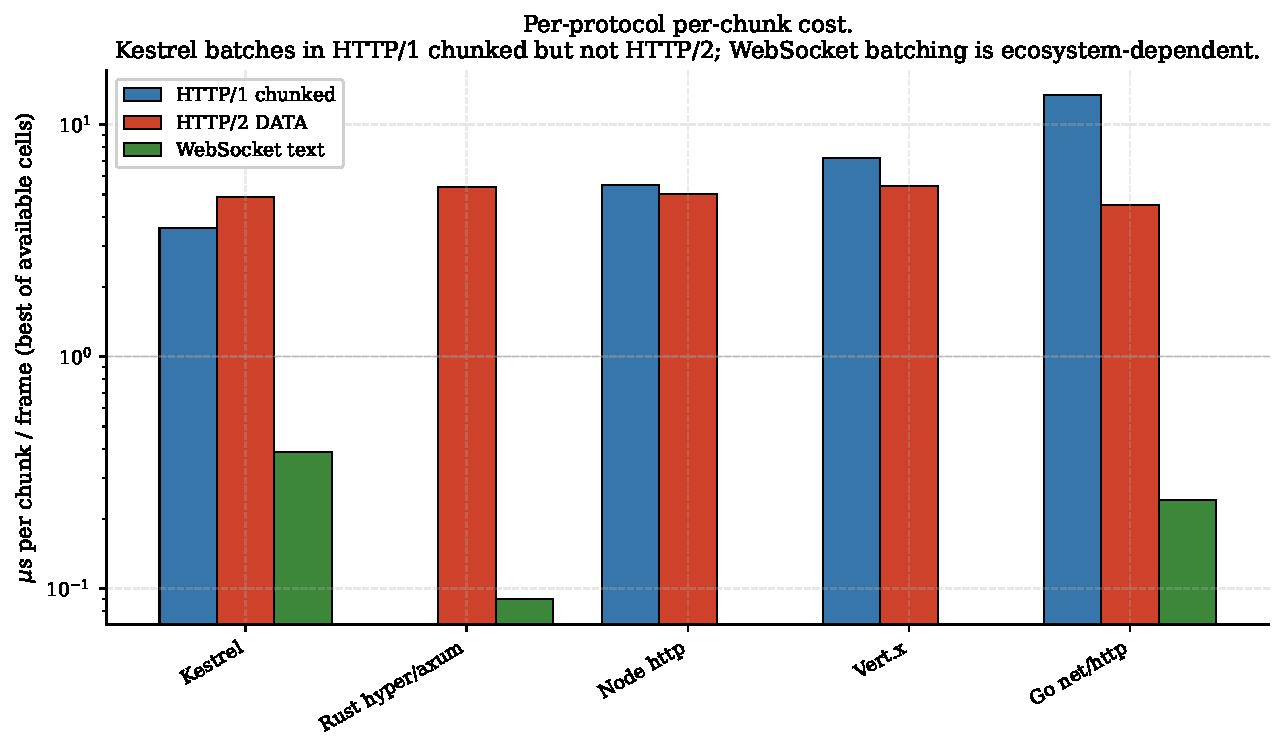
\includegraphics[width=\linewidth]{figures/protocol_compare.pdf}
  \caption{Per-protocol per-chunk-or-frame cost for servers
  measured in at least two of (HTTP/1 chunked-TE, HTTP/2 DATA,
  WebSocket text frame). Log-scale y. Kestrel batches in
  HTTP/1 but not HTTP/2; node-ws, gorilla, tungstenite, and
  Kestrel-WS batch in WebSocket but their HTTP/1 counterparts
  do not. The batching behavior is per-protocol-implementation,
  not per-server-author.}
  \label{fig:protocol-compare}
\end{figure}
